\chapter{Conclusion}
This chapter will give a short summary of the whole project and its findings.
The first section starts by reviewing what has been done while the second section will then bring up some aspects where the \gls{icds} could be improved to yield results either faster or more accurate.

\section{Summary}
The aim of this project was to find ways of unveiling whether an IMSI catcher is being operated in the close perimeter or not.
In other words to find out if it is safe to connect to the GSM network.
An unsafe environment could result in IMSI numbers being requested and saved by IMSI catchers or in phone calls being recorded.
The main premise that distinguishes this project from other similar projects like the also  OsmocomBB based 'Catcher Catcher' is that the system is operating in a completely passive manner.
Therefore it can only work on a limited amount of information, namely on information that is broadcasted on publicly available channels.
The benefit this yields over other projects is that the IMSI Catcher Detection System itself is completely invisible to the IMSI catcher.

Chapter 2 laid out basic concepts of \gls{gsm} communication to create a basis for understanding why and how an IMSI catcher works.
Some more detailed concepts on the $U_m$ interface were discussed to enable the reader to grasp the concept of logical channels and how they can be used to harvest information in a passive manner.
The chapter concluded with an account of how an IMSI catcher operates by outlining the two main ways of attacking a subscriber --- one by creating a new cell for the subscriber to connect to and the other by overtaking an already existent cell.

Chapter 3 started by explaining how the OsmocomBB framework was used to build the \gls{icds}.
It concluded with a summary of how to configure and use the system.
The two main sources of information, the \gls{bcch} and the \gls{pch} were introduced along with the different parameters that the \gls{icds} bases its findings on.
An outline of how this finding is reached is illustrated in Figure \ref{fig:decision_process}.
At first a sweep scan is conducted or an old project is loaded to supply the \gls{icds} with information of the surrounding base stations.
During the scan or after the data has been loaded the \gls{icds} evaluates different rules on the data.
This can be done with or without consulting databases containing local information.
\begin{figure}
\centering
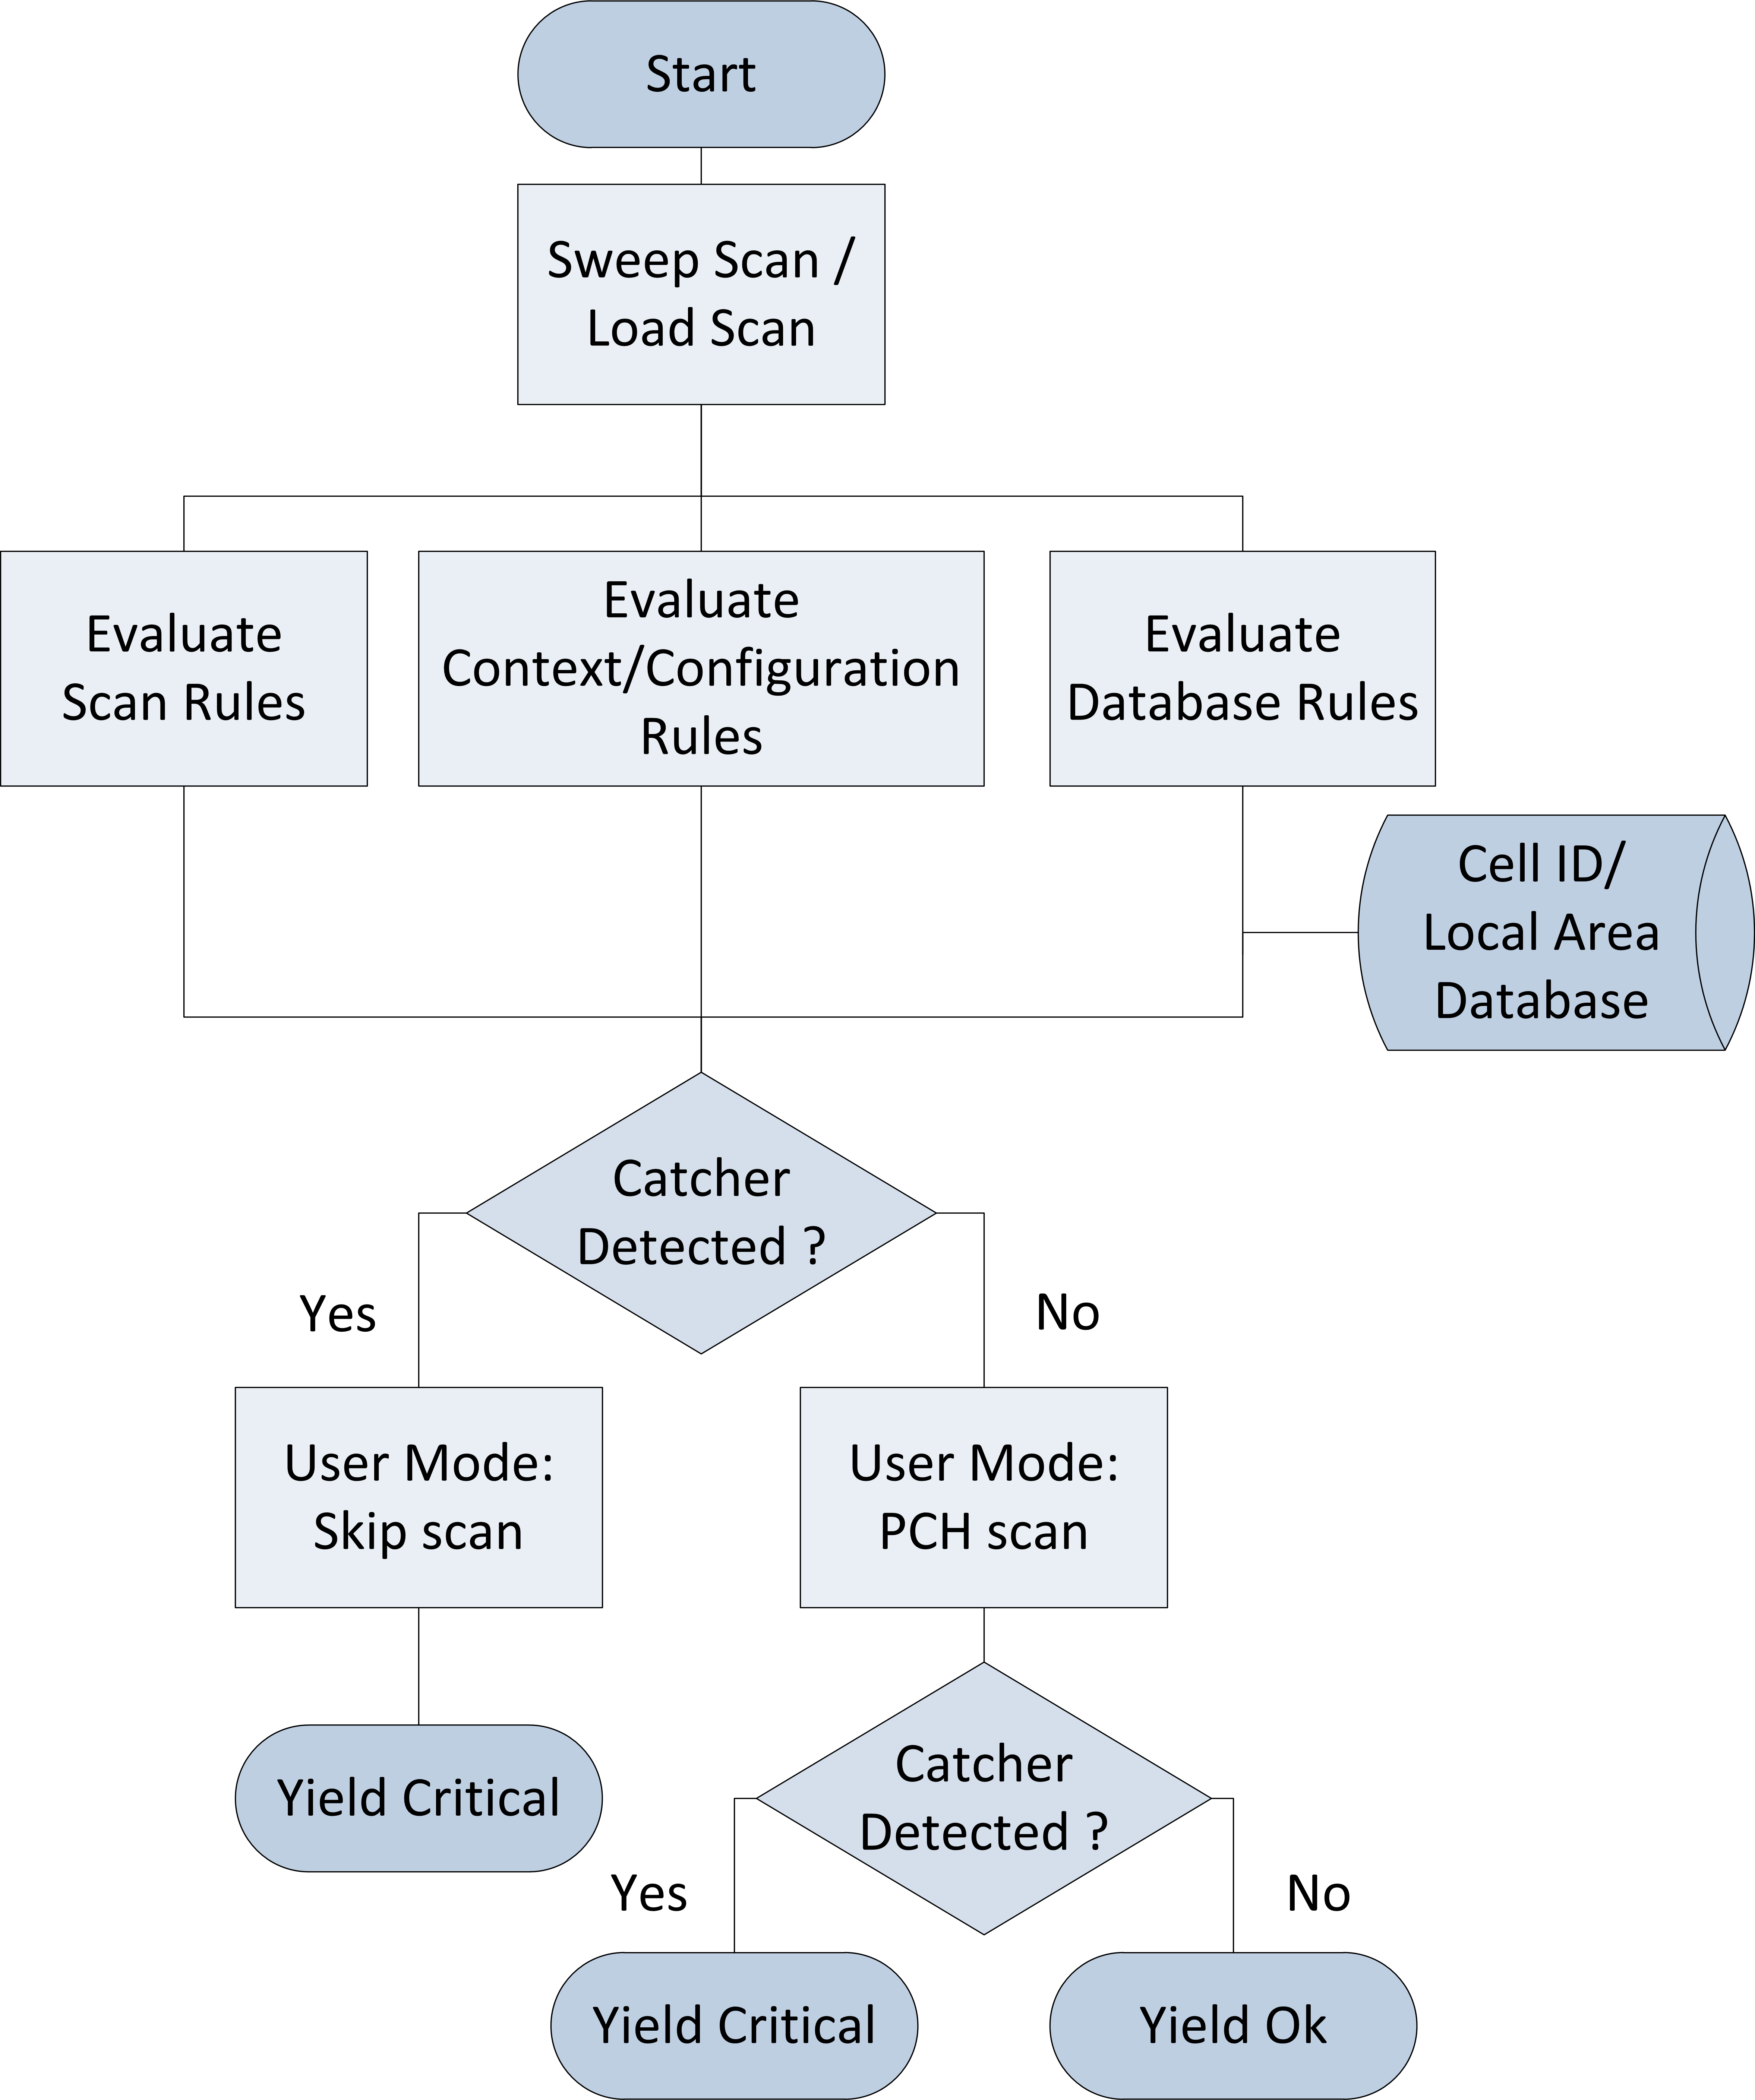
\includegraphics{../Images/flowchart}
\caption{ICDS decision finding process outlined.}
\label{fig:decision_process}
\end{figure}
The results show that some IMSI catcher configurations can be uncovered by these rules which check basic configuration data obtained from System Information messages.
In addition to this data broadcasted on the \gls{bcch}, reception levels and \glspl{lac} are also monitored over time to unveil attacks in which existing base stations are replaced by IMSI catchers.
This leaves IMSI catchers that have a consistent configuration and blend well in their surroundings concerning the reception levels.
They are also broadcasting the same \gls{lac} as the replaced base station, even if this means it could take a long time until the \gls{ms} announces itself.
To handle this case the \gls{icds} can monitor the \gls{pch} of the base station in question to gather Paging Messages and Immediate Assignments.
Since an IMSI catcher is not part of the provider's network no Paging Messages will be forwarded to the connected subscribers.
These findings have been confirmed with the experiments in Chapter 4 where different attack scenarios have been tested.
In cases where the \gls{icds} was not able to uncover the IMSI catcher by rule evaluation the \gls{pch} scan yielded the desired result.
It should be kept in mind that the evaluation has been done against a prototype IMSI catcher since data from a real IMSI catcher is not available.
However the results provided in this thesis are based more on general procedures, the \gls{gsm} protocol itself and not tailored to the specific system.
Therefore they should be applicable to any IMSI catcher that uses the attacks outlined here.

\section{Future Work}
There are several ways in which the \gls{icds} could be improved.
The experiments showed that one of the main issues is the duration of the sweep scans.
If a \gls{bts} is replaced right after it has been scanned it can take up to seven minutes until it is scanned again and the IMSI catcher is uncovered.
That is the time that is needed to do a complete sweep scan.
The \gls{icds} could be refined so that only base stations of a particular provider are monitored so the duration of sweep scans is cut down, this could also be done upon entering \emph{User Mode}.

In case of the Open Source IMSI-Catcher no Paging Messages were sent.
However it would be possible for a catcher that is aware of this evaluation criterion to send fake Paging Messages to arbitrary \glspl{tmsi} to deceive the \gls{icds}.
To face this the \gls{icds} could be extended.
Since Paging Messages would be unreliable in such a case one would have to use \glspl{ia}.
The experiments have shown that this might increase scanning time on the \gls{pch} since these messages are much more rare than Paging Messages.
An \gls{ia} sent to a subscriber contains the dedicated channel on which the conversation between the base station and the mobile phone is to continue.
At this point the \gls{icds} already uses the information about dedicated channels to see whether frequency hopping is used or not.
If an \gls{ia} is caught by the \gls{icds} one could follow on the assigned channel and catch the Cipher Mode Message.
Since an IMSI catcher will disable encryption to tap into calls, the Cipher Mode Message would contain A5/0 as its encryption algorithm instead of A5/1 which is used in Germany.
This feature could be used to handle cases of fake Paging Messages or \glspl{ia}, however it would take longer to conduct the \gls{pch} scan.
Another problem would be that it requires another subscriber that is connected to the IMSI catcher initiating a call.
On the other hand a regular base station using encryption can also be verified this way.

These approaches are not strictly passive since they require another participant to become active.
Although not strictly passive the \gls{icds} would still be invisible thus fulfilling the premise of not being uncovered itself.

